\documentclass[UTF8,twoside]{ctexart}

\usepackage{amsmath}
\usepackage{amssymb}
\usepackage{fancybox}
\usepackage{fancyhdr}
\usepackage{color}
\usepackage{bibentry}
\usepackage{multirow}
\usepackage[CJKbookmarks=true]{hyperref}
\usepackage{tikz}
\usepackage{mathrsfs}
\usepackage{bm}
\usepackage[version=3]{mhchem}

\newtheorem{theo}{定理}[section]

\makeatletter % `@' now normal 'letter'
\@addtoreset{equation}{subsection}
\makeatother % `@' is restored as 'non-letter'
\makeatletter % `@' now normal 'letter'
\@addtoreset{figure}{section}
\makeatother % `@' is restored as 'non-letter'
\renewcommand\theequation{\oldstylenums{\thesubsection}%
.\oldstylenums{\arabic{equation}}}
\renewcommand\thefigure{\oldstylenums{\thesection}%
.\oldstylenums{\arabic{figure}}}

\DeclareMathOperator{\res}{Res}

\begin{document}
\setcounter{section}{3}
\title{现代量子力学}
\author{Laserdog}

\maketitle
\thispagestyle{empty}

\cleardoublepage
\pdfbookmark[1]{目录}{anchor}
\tableofcontents
\clearpage
\section{量子力学中的对称性}

\noindent 考虑到我们已经详尽的学习了转动理论,我们现在显然要讨论更一般的关于“对称性”,“简并”,和“守恒律”的内容。之所以把这么重要的内容推迟到现在讨论,是因为我们想用上第三章学的转动对称的知识,把它作为学习上的一个例子。
%\begin{comment} 在详尽的学习了转动理论之后,我们现在可以从更一般的角度来讨论“对称性”,“简并”,和“守恒律”三者之间的联系。\end{comment}
\subsection{对称性,守恒律,简并}


\noindent \\

\noindent \fbox{%
  \parbox{\textwidth}{%
    \begin{centering}
      {\textbf{本节框架}}\\
      本节通过对讲点理学里面的对称性与守恒律的关系开始引入对称性的作用,从而逐步引入量子力学里面的对称性,介绍对称算符的概念并讲了它的性质,同时结合了上一章,以转动能级的简并为例子引入了简并对应的对称性(具体内容会在第5章说明)。接下来讲了库伦势(或推广至一次反比势能)的SO(4)对称性,引入了新情况的生成元和4维的转动,从而体现了整个系统的良好的性质。
    \end{centering}
  }%
}  \\

\


\noindent {\textbf{经典物理中的对称性}}

\noindent 我们从对经典物理中的对称性和守恒律的概念做一个基本的回顾。在拉格朗日体系下的量子力学,我们先看拉格朗日量$L$:这是一个有关广义坐标$q_i$,和相应的广义速度$\dot{q}_i$的函数。如果$L$在如下置换中保持不变:

\begin{equation} \label{4.1.1}
q_i\rightarrow q_i + \delta q_i
\end{equation}

\noindent 那么我们就必须有

\begin{equation}
\frac{\partial{L}}{\partial{q_i}} = 0
\end{equation}

\noindent 接下来,根据拉格朗日方程,$d/dt(\partial L/\partial \dot{q}_i) - \partial L /\partial q_i = 0$,有

\begin{equation}
\frac{dp_i}{dt} = 0
\end{equation}

\noindent 其中正则动量定义为

\begin{equation}
p_i = \frac{\partial L}{\partial \dot{q}_i}
\end{equation}

\noindent 如果拉格朗日量$L$在({\ref{4.1.1}})中的变换下保持不变,那么相应的$q_i$所对应的正则动量,就成为了守恒量。

类似的,在哈密顿力学体系下,哈密顿量$H$看为是广义坐标$q_i$和广义动量$p_i$的函数,我们有

\begin{equation}
\frac{dp_i}{dt} = 0
\end{equation}

\noindent 每当

\begin{equation}
\frac{\partial H}{\partial q_i} = 0
\end{equation}

\noindent 所以,如果哈密顿量并不显含$q_i$的话,换句话说$H$具有在$q_i \rightarrow q_i + dq_i$的对称性的话,我们就有了守恒的量。\\

\noindent {\textbf{量子力学中的对称性}}

\noindent 在量子力学中我们已经学习了一个{\textbf{Unitary 算符}}\footnote[1]{如同上几章强调过的,我打算以后都写成Unitary 算符来代替酉算符,因为这个翻译太蠢了},比如说$\mathscr{G}$,如何与平移、转动算符建立关系。习惯来讲会把$\mathscr{G}$叫成一个{\textbf{对称算符}}不管它是否是一个物理体系自身展现的对称性所对应的算符。更进一步,我们学过了对称算符在无穷小变化下与identity\footnote[2]{就是不变换,保持自身的单位算符}的差异,我们可以写出

\begin{equation}
\mathscr{G} = 1 - \frac{i\epsilon}{\hbar}G
\end{equation}

\noindent 其中 $G$ 是这个问题中对称性算符的厄米生成元。我们现在假定$H$在$\mathscr{G}$下保持不变,那么就有

\begin{equation}
\mathscr{G}^{\dagger} H \mathscr{G} = H
\end{equation}

\noindent 这就相当于

\begin{equation} \label{4.1.9}
\left[G, H\right] = 0
\end{equation}

\noindent 根据海森堡的动力演化方程,我们有

\begin{equation} \label{4.1.10}
\frac{dG}{dt} = 0
\end{equation}

\noindent 因此,$G$是一个动力学常数。比方说,哈密顿量$H$在平移下保持不变,那么动量相应的就是一个动力学常数。

当$G$和$H$对易的时候,一个很有意义的做法是,从$G$的本征矢的角度来简单的回顾一下({\ref{4.1.9}})与$G$守恒之间的关系。假定在$t_0$时间,系统处于$G$ 的本征态,那么这个态之后的演化可以有时间演化算符来描述:

\begin{equation}
\left|g', t_0; t\right\rangle = U\left(t, t_0\right)\left|g'\right\rangle
\end{equation}

\noindent 这同样还是$G$的具有相同本征值$g'$的本征态。换句话说,一旦一个态矢是$G$的本征态,他就将会一直是$G$ 的本征态且具有相同的本征值。当然,这个证明在考虑到({\ref{4.1.9}})和({\ref{4.1.10}})同样表明了$G$与时间演化算符对易,即

\begin{equation}
G\left[U\left(t, t_0\right)\left|g'\right\rangle\right] = U\left(t, t_0\right)G\left|g'\right\rangle = g' \left[U\left(t, t_0\right)\left|g'\right\rangle\right]
\end{equation}
\\

\noindent {\textbf{简并}}

\noindent 我们现在来看看有关简并的概念。尽管简并可以很大程度的在经典力学的程度内进行讨论 -- 比如,讨论闭合无进动轨道的开普勒问题 (Goldstein 2002)\footnote[3]{Goldstein, Herbert, et al. "Classical mechanics." American Journal of Physics 70.7 (2002): 782-783.} -- 这个概念在量子力学中其实起着更重要的左右。我们假定下列关系

\begin{equation}
\left[H, \mathscr{G}\right] = 0
\end{equation}

\noindent 对于一些特定的对称算符,在能量$E_n$的本征基矢$\left|n\right\rangle$下成立。

\noindent 那么,$\mathscr{G}\left|n\right\rangle$同样也是能量本征态且具有相同的能量,因为

\begin{equation}  \label{4.1.14}
H\left(\mathscr{G}\left|n\right\rangle\right) = \mathscr{G}H\left|n\right\rangle = E_n \left(\mathscr{G}\left|n\right\rangle\right)
\end{equation}

\noindent 现在假定$\left|n\right\rangle$和$\mathscr{G}\left|n\right\rangle$表示不同的态。那么,这两个态具有相同的能量 -- 这就是说它们简并。通常来说这类$\mathscr{G}$由连续的参数来标记,比如说$\lambda$,表面对于所有的态,$\mathscr{G}\left(\lambda\right)\left|n\right\rangle$ 都具有相同的能量。

我们现在特别的来考虑转动,假定哈密顿量是转动不变的,我们有

\begin{equation}
\left[\mathcal{D}\left(R\right), H\right] = 0
\end{equation}

\noindent 这立马就表明了

\begin{equation}
\left[{\textbf{J}}, H\right] = 0,\ \ \ \left[{\textbf{J}}^2, H\right] = 0
\end{equation}

\noindent 我们于是就建立了$H,\  \textbf{J}^2,\  \textbf{J}_{z}$的共同本征态,用$\left|n; j, m\right\rangle$来标记。那么我们就得到了所有的

\begin{equation}
\mathcal{D}\left(R\right)\left|n; j, m\right\rangle
\end{equation}

\noindent 拥有同样的能量。我们在第3章中看到,在转动变换下不同的$m$值被“混在了一起”。总的来说,$\mathcal{D}\left(R\right)\left|n; j, m\right\rangle$ 是一个关于$2j + 1$个线性无关的态的线性组合。准确地讲就是

\begin{equation}
\mathcal{D}\left(R\right)\left|n; j, m\right\rangle = \sum_{m'} \left(R\right)\left|n; j, m‘\right\rangle \mathcal{D}^{\left(j\right)}_{m'm}\left(R\right)
\end{equation}

\noindent 然后,通过改变那个表示转动情况的连续的参数,对应的$\mathcal{D}\left(R\right)$,我们可以得到不同的关于$\left|n; j, m‘\right\rangle$ 的线性组合。如果对于任意一个$\mathcal{D}\left(R\right)$,所有的具有$\mathcal{D}\left(R\right)\left|n; j, m\right\rangle$ 形式的态都有相同的能量,那我们就可以说所有的具有不同的$m$的$\left|n; j, m\right\rangle$都具有相同的能量。所以这里的简并是$(2j+1)$重的,即是$m$所有可能选取值的个数。这一点同样可以通过如下方式直观的得出:不同的$m$的态可以利用升降算符$J_{\pm}$得到,而升降算符是和$H$对易的,所以$\left|n; j, m\right\rangle$具有相同的能量。

作为一个对对称性的应用,我们考虑一个原子中的电子,它的势能可以写作$V(r)+V_{LS}\bm{L \cdot S}$。因为$r$和$\bm{L\cdot S}$都是旋转不变的,我们期待每个原子能级有一个$(2j+1)$重的简并。另一方面,假定这里有外加电场或者磁场,比如$z$方向。旋转对称性如今显得被破坏了,所以不太可能有$(2j+1)$重简并了,而且不同的$m$对应的态也不太可能有相同的能量。我们将在第5章来检验这种分裂是如何产生的。\\

\noindent {\textbf{库伦势中的SO(4)对称性}}

\noindent 一个非常合适的关于量子力学的连续对称性的例子就是氢原子库伦势问题。我们在第3章第7节曾讨论过这个问题,在那里我们发现在式({\ref{3.7.53}})中的能量本征值极强的表现了({\ref{3.7.56}})中的简并。如果体系的简并是偶然的那将会更引人注目,但是实际上,这是由于$1/r$ 势的束缚态所有的附加对称性。

经典问题中,这种势的轨道,即开普勒问题,在量子力学之前就已经被仔细的研究过了。至于椭圆轨道是闭合的意味着应该有一些(矢量)运动常数来维持椭圆轨道的主轴方向。我们知道,即使是相比于$1/r$的一个小偏移都会导致主轴的进动,所以我们期望找到一个$1/r$势独特的运动常数。

经典的来说,这个常数是

\begin{equation}  \label{4.1.19}
\bm{M} = \frac{\bm{p\times L}}{m} - \frac{Ze^2}{r}\bm r
\end{equation}

\noindent 我们使用了在第3章第7节中使用过了的记号。这个常数矢量实际上被称为“伦茨矢量”,或者“伦格-伦茨矢量”\footnote[4]{$Runge-Lenz\  vector$}。 不想经典力学那样处理它,我们在量子框架下的对称性的手段来处理这个运动常数。

这个新的对称性,我们称之为SO(4),与我们在第3章第3节学到的SO(3)是完全类似的。这就是说,SO(4)是一个$4\times4$ 的转动矩阵,也就是说这是一个自正交的行列式为$1$的矩阵。我们接下来建立这种对称性的性质从而让伦茨矢量作为一个运动常数,然后我们会发现这些性质就是我们期待的SO(4) 的性质。

我们的接下来的推导与 Schiff (1958), pp. 235 - 39。我们首先需要修改({\ref{4.1.19}})来构建一个厄米算符。首先,对于两个厄米算符$\bm A$和$\bm B$,很显然的看到$\bm {A\times B}^{\dagger} = -\bm{B\times A}$。因此,伦茨矢量的厄米形式应该是

\begin{equation}
\bm {M} = \frac{1}{2m}\left(\bm{p\times L - L\times p}\right) - \frac{Ze^2}{r}\bm{r}
\end{equation}

\noindent 可以发现$\bm M$和哈密顿量:

\begin{equation}
H = \frac{\bm{p}^2}{2m} - \frac{Ze^2}{r}
\end{equation}

\noindent 对易,即

\begin{equation}
\left[\bm{M}, H\right] = 0
\end{equation}

\noindent 所以$\bm M$是一个(量子力学下的)运动常数。其它常用的与之相关的结论可以写作

\begin{equation}  \label{4.1.23}
\bm{L \cdot M} = 0 = \bm{M \cdot L}
\end{equation}

\begin{equation}  \label{4.1.24}
\text{和}\ \ \ \ \bm{M}^2 = \frac{2}{m}H\left(\bm{L}^2 + \hbar^2\right) + Z^2e^4
\end{equation}

为了找到这个运动常数对应的对称性,一个有指导意义的做法是回顾一下代数里面学到的对称性的生成元。我们已知了一些代数形式:

\begin{equation}  \label{4.1.25}
\left[L_i, L_j\right] = i\hbar \epsilon_{ijk}L_k
\end{equation}

\noindent 我们曾在(\ref{3.6.2})中写过这种表达,要对重复的指标(这里就是$k$)进行求和\footnote[5]{译注:为了防止没看懂(真的会有人没看懂吗?),等式右边实际上相当于\\ \[\sum_k i\hbar \epsilon_{ijk}L_k\]}。我们同样可以得到

\begin{equation}  \label{4.1.26}
\left[M_i, L_j\right] = i\hbar \epsilon_{ijk}M_k
\end{equation}

\noindent 这实际上把$\bm M$树立成一个和(\ref{3.11.8}) 一样的矢量算符。而最后,我们还可以得到

\begin{equation}  \label{4.1.27}
\left[M_i, M_j\right] = -i\hbar \epsilon_{ijk}\frac{2}{m}HL_k
\end{equation}

为了明确一下,(\ref{4.1.25}),(\ref{4.1.26})和(\ref{4.1.27})并不构成闭合的代数对易关系,由于(\ref{4.1.27})中出现了$H$,所以这使得把这些算符作为连续对称性系统的生成元不现实。但是,我们可以考虑一个特殊的束缚体系。在这个情况下,向量空间被减小到只针对那些$H$的本征态,且本征值$E < 0$。这样的话我们就能在(\ref{4.1.27})中用$E$替代$H$了,这样就有了闭合的对易关系。为了形式上看的更对称,引入一个正比于$\bm M$ 的矢量算符

\begin{equation}  \label{4.1.28}
\bm N \equiv \left(-\frac{m}{2E}\right)^{1/2}\bm M
\end{equation}

\noindent 所以,我们拥有如下闭合的代数对易关系:

\begin{subequations}  \label{4.1.29}
\begin{align}
\left[L_i, L_j\right] = i\hbar \epsilon_{ijk}L_k \\
\left[L_i, L_j\right] = i\hbar \epsilon_{ijk}L_k \\
\left[L_i, L_j\right] = i\hbar \epsilon_{ijk}L_k
\end{align}
\end{subequations}

所以我们在(\ref{4.1.29})中利用$\bm{L, N}$生成的对称性是什么呢?尽管很不显然,但这个问题的答案是“四维空间的旋转”。首先的线索就是生成元的数量,6 个,每一个都相当于对应一些轴的转动。把转动想象为一些把两个轴进行“混合”的操作,相应的,在一定维度的空间中生成元的数量应该是$n(n-1)/2$。 由此,而2维的转动就有1个生成元,3维的转动就有3个生成元,4维的转动就有6个生成元。

想要看出(\ref{4.1.29})实际上是一个恰当的四维转动的代数结构就更困难了,但是我们换一个角度考虑。在三维空间中,轨道角动量算符({\ref{3.6.1}})生成了转动操作。我们从(\ref{3.6.6})中看的更清楚,对于$\left|\alpha\right\rangle$的一个绕着$z$轴的无穷小转动可以用$\left|x, y, z\right\rangle$ 来表示。之所以能这样,是因为动量算符可以看做空间评议的一个生成元。事实上,如$L_z = xp_y - yp_x$这样坐标和动量的组合形式相当于把$x, y$两个轴进行了“混合”,就像我们希望的绕$z$轴的转动生成元所做的那样。

为了推广这一性质到四维空间,我们首先用$(x_1, x_2, x_3),\ (p_1, p_2, p_3)$来替代$(x, y, z),\ (p_x, p_y, p_z)$。从而,我们就需要重新写生成元,就像$L_3 = \tilde{L}_{12} = x_1p_2 - x_2p_1,\ \ L_1 = \tilde{L}_{23},\ \ \text{和}\ L_2 = \tilde{L}_{31}$。 如果我们接下来开发一个新的空间坐标$x_4$和相应的共轭动量$p_4$(之间满足正常的坐标-动量对易关系),我们可以定义:

\begin{subequations}  \label{4.1.30}
\begin{align}
\tilde{L}_{14} = x_1p_4 - x_4p_1 \equiv N_1\\
\tilde{L}_{24} = x_2p_4 - x_4p_2 \equiv N_2\\
\tilde{L}_{34} = x_3p_4 - x_4p_3 \equiv N_3
\end{align}
\end{subequations}

\noindent 这样一来很容易就看出$N_1$符合(\ref{4.1.29}) 规定的代数关系,例如:

\begin{equation}
\begin{split}
\left[N_1, L_2\right] &= \left[x_1p_4 - x_4p_1, x_3p_1 - x_1p_3\right]\\
&=p_4\left[x_1, p_1\right]x_3 + x_4\left[p_1, x_1\right]p_3\\
&=i\hbar\left(x_3p_4 - x_4p_3\right) = i\hbar N_3\\
\end{split}
\end{equation}

\noindent 换句话说,这就是四维空间的代数对易形式。不过在继续研究之前,我们先稍微看看(\ref{4.1.14})指出的库伦势的简并:

定义算符

\begin{align}
\bm{I} \equiv \bm{(L + N)}/2  \\
\bm{K} \equiv \bm{(L - N)}/2
\end{align}

\noindent 我们可以很简单的证明如下对易关系:

\begin{subequations}  \label{4.1.34}
\begin{align}
\left[I_i, I_j\right] &= i\hbar\epsilon_{ijk}I_k\\
\left[K_i, K_j\right] &= i\hbar\epsilon_{ijk}K_k\\
\left[I_i, K_j\right] &= 0
\end{align}
\end{subequations}

\noindent 因此,这些算符遵守各自独立的叫动量对易关系。同时,很显然的也有$\left[\bm{I}, H\right] = \left[\bm{K}, H\right] = 0$。因此,这些“角动量”们是守恒律,并且我们知道$\bm{I}^2, \text{和}\bm{K}^2$的本征值分别是$i(i+1)\hbar^2,\ k(k+1)\hbar^2$,其中$i, k = 0, \frac{1}{2}, 1, \frac{3}{2}, \cdots$

根据(\ref{4.1.23})和(\ref{4.1.28}),$\bm{I^2 - K^2} = \bm{L \cdot N} = 0$,我们必须让$i = l$才行。而另一方面,算符

\begin{equation}
\bm{I^2 + K^2} = \frac{1}{2}\left(\bm{L^2 + N^2}\right) = \frac{1}{2}\left(\bm{L^2} - \frac{m}{2E}\bm{M^2}\right)
\end{equation}

\noindent 由此,结合(\ref{4.1.24}),得到

\begin{equation}
2k(k+1)\hbar^2 - \frac{1}{2}\left(-\hbar^2 - \frac{m}{2E}Z^2e^4\right)
\end{equation}

\noindent 解出$E$,我们有

\begin{equation}
E = -\frac{mZ^2e^4}{2\hbar^2}\frac{1}{(2k+1)^2}
\end{equation}

\noindent 这与(\ref{3.7.53})一致,只是把主量子数$n$改成了$2k+1$而已。我们现在看到,库伦势的“对称性”主要源于两个算符$\bm{I, K}$所表达的那种“转动”对称性。这个对称性的简并度是$(2i+1)(2k+1) = (2k+1)^2 = n^2$。这个(\ref{3.7.56})所得到的一样,只不过这回我们明确了这种简并并不是偶然而是有原因的。

如果我们不去真的求解氢原子的薛定谔方程,那么我们刚才所解的这一系列东西实际上都没有意义。相反的,我们充分的利用了内部的对称性来得到更多相同的答案。这个解由泡利\footnote[6]{Pauli}最先给出。

用节{\ref{S3.3}}中我们了解了一点的连续群理论的语言来说,我们看到(\ref{4.1.29})的代数对易关系与SO(4)群相联系。不仅如此,在(\ref{4.1.34})中重写的形式可以看出来这个可以被看做是两个独立的SU(2)群 -- 即SU(2)$\times$SU(2)群。尽管本书在这里的目的并不是做一个群论的概论说明,我们还是要更深入的讲一下一个$n$ 维空间的转动如何表示 -- SO(n)群。

将节{\ref{S3.3}}进行一般化,考虑一个$n\times n$的正交矩阵\footnote[7]{不确定中文叫啥。。就是自己和自己的转置正交}$R$组成的群来表示$n$ 维的转动。它们可以用参数描述成这样:

\begin{equation}
R = \exp\left(i\sum_{q = 1}^{n(n - 1)/2}\phi^q \tau^q\right)
\end{equation}

\noindent 其中$\tau^q$是纯虚的,且是反对称的矩阵,即,$\left(\tau^q\right)^T = -\tau^q$\footnote[8]{竟然在试读的时候有人问我这个$\tau^q$上的$T$ 次方是啥。。我也是醉了,这是转置},$\phi^q$是广义旋转角。反对称性质保证了$R$是正交矩阵,系数$i$表示了纯虚的$\tau^q$也能构成厄米矩阵。

显然的,$\tau^q$与转动算符生成元密切相关。事实上,是它们的对易关系应该来模仿生成元们的对易关系。依照节{\ref{S3.1}}的做法,我们比较绕$p$轴且绕$q$ 轴的无穷小旋转的先后带来的差异,即

\begin{equation} \label{4.1.39}
\begin{split}
\left(1+i\phi^p\tau^p\right)\left(1+i\phi^q\tau^q\right) - & \left(1+i\phi^q \tau^q \right) \left(1+i\phi^p\tau^p\right)\\
&=-\phi^p\phi^q\left[\tau^p, \tau^q\right]\\
&=1-\left(1+i\phi^p\phi^q\sum_r f_r^{pq}\tau^r\right)
\end{split}
\end{equation}

\noindent (\ref{4.1.39})的最后一行说明了这个结果必然是绕两个轴转动生成元的二阶项的一些线性组合。$f_r^{pq}$叫做转动群的{\it{结构常数}}。它能给出对易关系:

\begin{equation}
\left[\tau^p, \tau^q\right] = i\sum_r f_r^{pq} \tau^r
\end{equation}

\noindent 接下来更深入的研究就是去确定这些结构常数,不过我们就把这个内容留给专门讲授群论的书吧。不过,对于三维问题,我们倒是不难给出$f_r^{pq} = \epsilon_{pqr}$,就像我们直觉感觉的那样。

\subsection{分立对称性,宇称,或空间反演}\label{Sec4.2}


\noindent \\

\noindent \fbox{%
  \parbox{\textwidth}{%
    \begin{centering}
      {\textbf{本节框架}}\\
      啊啊啊
    \end{centering}
  }%
}  \\

\


\noindent 到目前为止我们考虑了连续对称性算符 -- 即,可以通过施加连续的无限小的对称操作而得到的算符。不是所有的对称性操作在量子力学中都必然的有这种(连续的)形式的。这一节,我们来考虑三个可以称得上是“分立”而不是连续的对称性操作 -- 宇称、格点平移和时间反演。

我们考虑的第一个操作就是宇称变换,或者说是空间反演。宇称变换如果作用在坐标系下,则使得右手系(RH)变成左手系(LH),如图{\ref{Fig4.1}}。但是,我们本书中不考虑它作用在坐标系上,而是考虑它作用在一个态矢上。给定一个态$\left|\alpha\right\rangle$,考虑通过一个{\textbf{Unitary}}算符 -- 反演算符 -- $\pi$ 作用在它身上得到的它的空间反转态,如下:

\begin{equation}
\left|\alpha\right\rangle\ \rightarrow\ \pi\left|\alpha\right\rangle
\end{equation}

\noindent 我们需要这样的空间反转的情况下,$\bm x$的期望值应该取负。

\begin{equation}
\left\langle\alpha\right|\pi^{\dagger}\bm{x}\pi\left|\alpha\right\rangle =  -\left\langle\alpha\right|\bm{x}\left|\alpha\right\rangle
\end{equation}

\noindent 这是一个很合理的要求。如果有

\begin{equation} \label{4.2.3}
\pi^{\dagger}\bm{x}\pi = -\bm{x}
\end{equation}

\noindent 或者

\begin{equation}
\pi\bm{x} = -\bm{x}\pi
\end{equation}

\noindent 其中我们用到了$\pi$的{\textbf{Unitary}}性质。换句话说,$\pi$和$\bm{x}$必须反对易。

动量算符的本征态是如何在宇称算符下变换的呢?我们说

\begin{equation} \label{4.2.5}
\pi\left|\bm {x'}\right\rangle = e^{i\delta}\left|-\bm{x'}\right\rangle
\end{equation}

\noindent 其中$e^{i\delta}$是一个相因子($\delta$是实数)。为了证明这点,我们考虑

\begin{equation}
\bm{x} \pi \left|\bm {x'}\right\rangle = - \pi \bm{x} \left|\bm {x'}\right\rangle = (-\bm{x'})\pi \left|\bm {x'}\right\rangle
\end{equation}

\noindent 这个方程说明$\pi \left|\bm {x'}\right\rangle$也是$\bm x$算符的本征函数,本征值为$-\bm {x'}$,所以它等于坐标本征值$\left|\bm {-x'}\right\rangle$乘以一个相位因子而已。

通常取$e^{i\delta} = 1$。用这个代入(\ref{4.2.5}),我们有$\pi^2 \left|\bm {x'}\right\rangle = \left|\bm {x'}\right\rangle$。因此,我们有$\pi^2 = 1$,也就是说,如果我们对一个态作用两次$\pi$,它保持不变。我们从(\ref{4.2.5})中看出,$\pi$不仅是Unitary的,还是厄米的。



\begin{figure}
\begin{centering}
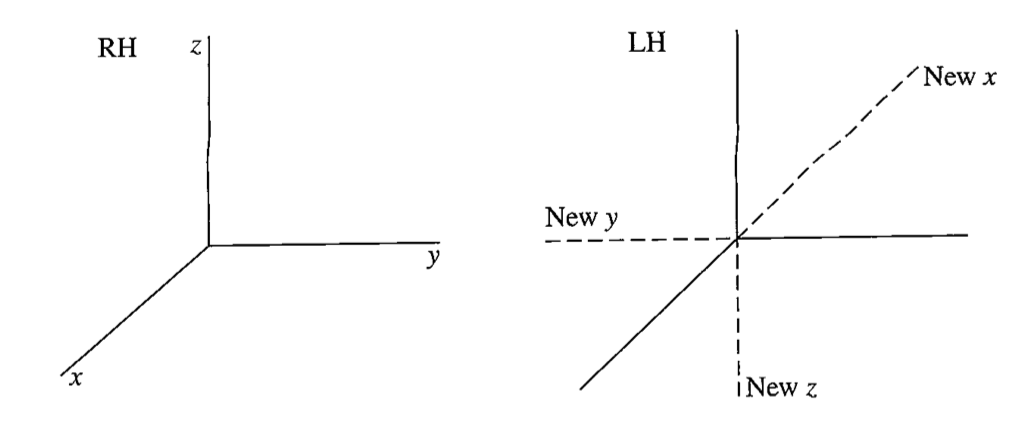
\includegraphics[width = 12.4cm]{./Sakurai/Fig_4.1.png}
\caption{右手系(RH)和左手系(LH)}
\label {Fig4.1}
\end{centering}
\end{figure}


\begin{equation}
\pi^{-1} = \pi^{\dagger} = \pi
\end{equation}

\noindent 它的本征值只能是$+1$和$-1$。

那么,动量算符呢?动量算符$\bm p$有点像$md\bm{x}/dt$,所以我们很自然的想象它在宇称变化下显现奇性,就像$\bm x$一样。一个更令人接受的观点是把动量算符看做平移这种操作的生成元。注意到跟在宇称变换后进行的平移操作,等于进行{\emph{反向的}}平移跟一个进行宇称变换\footnote{这里的先后指的是算符的位置,事实上“后”的算符先作用在右矢上},如图{\ref{Fig4.2}}所示。所以,

\begin{equation}
\pi \mathcal{T}(d\bm x') = \mathcal{T}(-d\bm x')\pi
\end{equation}
\begin{equation}
\pi \left(1 - \frac{\bm p \cdot d\bm x'}{\hbar}\right) \pi^{\dagger} = \left(1 + \frac{\bm p \cdot d\bm x'}{\hbar}\right)
\end{equation}

\begin{figure}
\begin{centering}
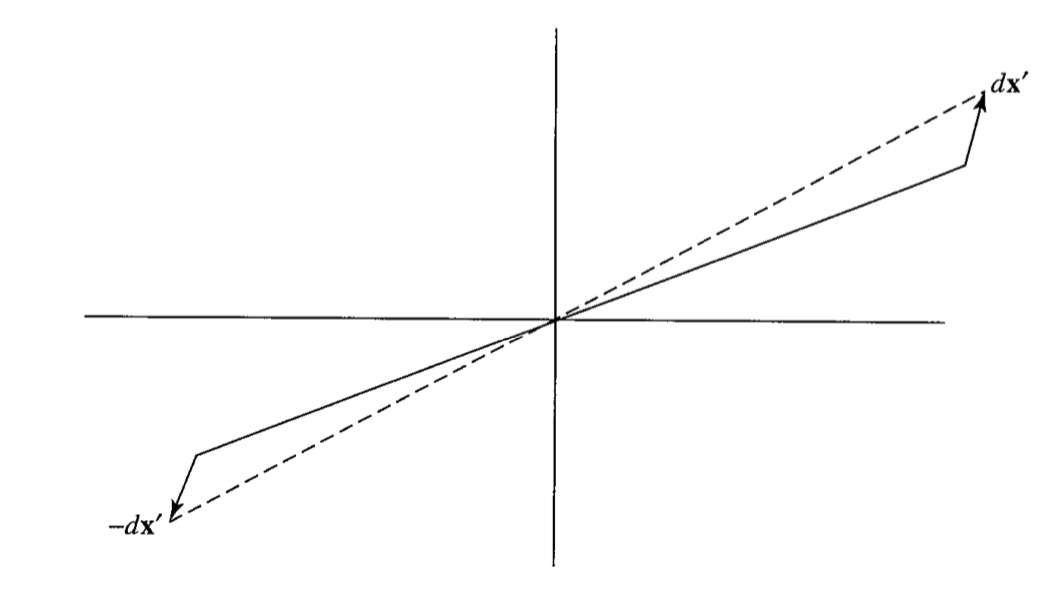
\includegraphics[width = 10cm]{./Sakurai/Fig_4.2.png}
\caption{先后进行的平移与宇称变换}
\label {Fig4.2}
\end{centering}
\end{figure}

\noindent 其中有

\begin{equation} \label{4.2.10}
\left\{\pi, \bm p\right\} = 0\ \ \ \ \text{或者}\ \ \ \ \pi^{\dagger} \bm{p} \pi = -\bm p
\end{equation}

我们现在讨论$\bm J$在宇称变化下的行为。首先,轨道角动量显然有

\begin{equation} \label{4.2.11}
\left[\pi, \bm L\right] = 0
\end{equation}

\noindent 因为

\begin{equation}
\bm{L = x\times p}
\end{equation}

\noindent 而且$\bm x$和$\bm p$都是奇宇称的。但是,为了看到这个性质同样适用于自旋,我们最好使用$\bm J$是转动生成元这个事实。对$3\times 3$正交矩阵,我们有

\begin{equation}
R^{\text{宇称}}R^{\text{旋转}} = R^{\text{旋转}}R^{\text{宇称}}
\end{equation}

\noindent 其中很明显的,

\begin{equation}
R^{\text{宇称}} = \begin{pmatrix}-1 & &0 \\  &-1 & \\ 0 & &-1 \end{pmatrix}
\end{equation}

\noindent 这就是说,宇称变换和转动是对易的。在量子力学里,假定对应的算符是Unitary的是一件很自然的事情,所以

\begin{equation} \label{4.2.15}
\pi \mathcal{D}(R) = \mathcal{D}(R) \pi
\end{equation}

\noindent 其中$\mathcal{D}(R) = 1 - i \bm{J}\cdot \hat{\bm n} \epsilon/\hbar$。从(\ref{4.2.15})中可以看到,

\begin{equation} \label{4.2.16}
\left[\pi, \bm{J}\right] = 0\ \ \ \ \text{或者} \pi^{\dagger}\bm{J}\pi = \bm{J}
\end{equation}

\noindent 这个,与(\ref{4.2.11})一起表明了自旋算符$\bm S$(构成了总角动量算符$\bm {J = L + S}$)与轨道角动量$\bm L$一样变换。

在旋转下,$\bm {x, J}$的变换方式一样,所以他们都是矢量,或者称为秩为$1$的球张量\footnote{关于球张量,可以参考节{\ref{S3.6}}的内容。}。但是,$\bm x \text{或}\bm p$在宇称变化下是奇性的[参见(\ref{4.2.3}),(\ref{4.2.10})],而角动量$\bm J$是偶性的[参看(\ref{4.2.16})]。我们把宇称变换下显奇性的叫做{\textbf{极矢量}},而把显偶性的叫做{\textbf{轴矢量}}或{\textbf{隗矢量}}。

我们现在考虑一个形如$\bm{S}\cdot\bm{x}$的算符。在旋转下,它们表现的像正常的标量一样,比如$\bm{S}\cdot\bm{L},\, \bm{x}\cdot\bm{P}$。但是在空间反演对称的情况下,我们有:

\begin{equation}
\pi^{-1} \bm{S}\cdot\bm{x}\pi = -\bm{S}\cdot\bm{x}
\end{equation}

\noindent 但是对于一般的标量满足

\begin{equation}
\pi^{-1} \bm{S}\cdot\bm{L}\pi = \bm{S}\cdot\bm{L}
\end{equation}


这样的关系。算符$\bm{S}\cdot\bm{x}$就是一个隗矢量的例子。

\ 

\noindent \textbf{从宇称看波函数}

\noindent 我们现在看一下波函数的宇称性质。首先,假定$\psi$是一个没有自旋,态矢量为$|\alpha\rangle$的粒子:

\begin{equation}
\psi(\bm{x}') = \langle\bm{x}'|\alpha\rangle
\end{equation}

\noindent 空间反演下的态,用$\pi|\alpha\rangle$来表示,就是

\begin{equation}
\langle\bm{x}'|\pi|\alpha\rangle = \langle\bm{x}'|\alpha\rangle = \psi(-\bm{x}')
\end{equation}

假定$|\alpha\rangle$是宇称算符的本征态。我们知道,宇称算符的本征值必须是$\pm 1$,所以,

\begin{equation}
\pi|\alpha\rangle = \pm|\alpha\rangle
\end{equation}

\noindent 我们可以看到,相应的波函数是

\begin{equation}
\langle\bm{x}'|\pi|\alpha\rangle = \pm \langle\bm{x'}|\alpha\rangle
\end{equation}

\noindent 但注意我们同样有:

\begin{equation} \label{4.2.23}
\langle\bm{x}'|\pi|\alpha\rangle = \langle-\bm{x}'|\alpha\rangle
\end{equation}

\noindent 所以态$|\alpha\rangle$是偶宇称或奇宇称,得看波函数是否满足:

\begin{equation} \label{4.2.24}
\psi(-\bm{x}') = \pm\psi(\bm{x}')
\begin{cases}
\text{even parity}\\
\text{odd parity}
\end{cases}
\end{equation}

并不是所有的物理上感兴趣的波函数都像(\ref{4.2.24})一样有明确的宇称。比方说,考虑动量本征函态。动量算符与宇称算符反对易,所以动量本征态绝对不是宇称算符的本征态。这确实可以从动量本征态的函数形式——平面波看出来,它并不符合(\ref{4.2.24})。

轨道角动量的本征态应当是宇称算符的本征态,因为$\bm{L}$和$\pi$是对易的[见(\ref{4.2.11})]。为了研究$\bm{L}^2$和$L_z$的共同本征态在宇称变换下变化,我们检验它的波函数在空间反演下的行为,

\begin{equation}
\langle\bm{x}'|\alpha,\, lm\rangle = R_{\alpha}(r)Y_l^m (\theta, \phi)
\end{equation}

\noindent 而$\bm{x}' \rightarrow -\bm{x}'$的变化是由

\begin{equation} \label{4.2.26}
\begin{split}
r&\rightarrow r\\
\theta&\rightarrow \pi - \theta\quad(\cos\theta\rightarrow-\cos\theta)\\
\phi&\rightarrow\phi+\pi\quad\left(e^{im\phi}\rightarrow(-1)^me^{im\phi}\right)
\end{split}
\end{equation}

利用球谐函数的具体形式,

\begin{equation}
Y_l^m = (-1)^m\sqrt{\frac{(2l+1)(l-m)!}{4\pi(l+m)!}}P_l^m(\cos\theta)e^{im\phi}
\end{equation}

\noindent 对于整的$m$,由(\ref{3.6.38}),其中

\begin{equation}
P_l^{|m|}(\cos\theta) = \frac{(-1)^{m+l}}{2^ll!}\frac{(l+|m|)!}{(l-|m|)!}\sin^{-|m|}\theta\left(\frac{d}{d(\cos\theta)}\right)^{l-|m|}\sin^{2l}\theta
\end{equation}

\noindent 我们可以明确的说

\begin{equation}
Y_l^m \rightarrow (-1)^lY_l^m
\end{equation}

\noindent 其中,$\theta$和$\phi$如(\ref{4.2.26})一样变换。因此,我们可以总结如下:

\begin{equation}
\pi|\alpha, lm\rangle = (-1)^l |\alpha, lm\rangle
\end{equation}

\noindent 事实上,这并不需要有类似于$Y_l^m$的项。一个更简单的能得到相同结果的办法是让$m=0$然后利用$L_{\pm}^r|l, m=0\rangle(r = 0, 1, \cdots, l)$必须拥有相同的宇称性,因为$\pi$和$(L_{\pm})^r$对易。

我们现在看看能量本征态的宇称如何,我们首先从一个重要的引理开始。

\begin{theo}
假定

\begin{equation}
\left[H, \pi\right] = 0
\end{equation}

\noindent 并且$|n\rangle$和$E_n$是一组$H$的非简并的本征态和本征值:

\begin{equation} \label{4.2.32}
H|n\rangle = E_n|n\rangle
\end{equation}

\noindent 那么,$|n\rangle$仍然是宇称算符的本征态。
\end{theo}

\noindent {\emph{证明}} 为了证明这个定理,我们首先注意到

\begin{equation} \label{4.2.33}
\frac{1}{2}(1\pm\pi)|n\rangle
\end{equation}

是本征值为$\pm 1$的宇称本征态(使用了$\pi^2 = 1$)。但是这同时也是能量算符的本征值为$E_n$的本征态。因为能级是非简并的,$|n\rangle$和(\ref{4.2.33})必须表示同一个态。于是就有$|n\rangle$,即(\ref{4.2.33})的一个常数倍,必然也是本征值为$\pm 1$的宇称本征态。

我们来看看简谐振子这个例子。它的基态,$|0\rangle$,是偶宇称的,因为它的波函数是高斯型的,满足$\bm{x}'\rightarrow-\bm{x}'$下的不变。它的第一激发态

\begin{equation}
|1\rangle = a^{\dagger}|0\rangle
\end{equation}

\noindent 必须是奇宇称的,因为$a^{\dagger}$是$x,\, p$的线性算符,而它们都是奇宇称的[见(\ref{2.3.2})]。一般的,简谐振子升算符得出的第$n$个激发态的宇称为$(-1)^n$。

值得注意的是,非简并性是这个论断的最基本的依据。比如,考虑氢原子的非相对论情况。此时,能量本征值取决于主量子数$n$(因此,像$2p$和$2s$态就是简并的了)——库伦势显然是宇称变换下不变的,但是能量本征值

\begin{equation}
c_p|2p\rangle + c_s|2s\rangle
\end{equation}

\noindent 则显然不是一个宇称本征态。

另一个例子可以想象动量本征态。动量与宇称算符是反对易的,所以,即便自由离子的哈密顿量$H$是于晨霞不变的,动量本征态(显然也是能量本征态),并不是宇称本征态。我们的定理仍然没有问题,是因为这里并没有满足我们定理要求的非简并,比如$|\bm{p}'\rangle$和$|-\bm{p}'\rangle$,就拥有相同的能量但却是不一样的态。其实,我们倒是可以很简单的根据这个做一个线性组合$(1/\sqrt{2})(|\bm{p}'\rangle\pm|-\bm{p}'\rangle)$:这是宇称算符的本征值$\pm 1$的一组本征态。用波函数的角度来说,$e^{i\bm{p}'\cdot\bm{x}'/\hbar}$并没有确切的宇称,但是$\cos \bm{p}'\cdot\bm{x}'/\hbar$和$\sin \bm{p}'\cdot\bm{x}'/\hbar$有(前者偶后者奇)。

\ \\

\noindent \textbf{对称双势阱}

\noindent 我们接下来考虑一个很基本但是有指导意义的例子:对称双势阱,如图{\ref{Fig4.3}}。哈密顿量显然是宇称变换下的不变量。最低的两个能态已经标在图{\ref{Fig4.3}}上,就如同我们精确解得的那样,在经典区域范围内是$\cos$和$\sin$形式,在紧点进去里面是$\sinh$和$\cosh$形式。解与时能不连续所对应,我们叫它{\textbf{对称态}}$|S\rangle$和{\textbf{反对称态}}$|A\rangle$。当然,他们自然是$H$和$\pi$的本征态。进一步计算给出

\begin{figure}
\begin{centering}
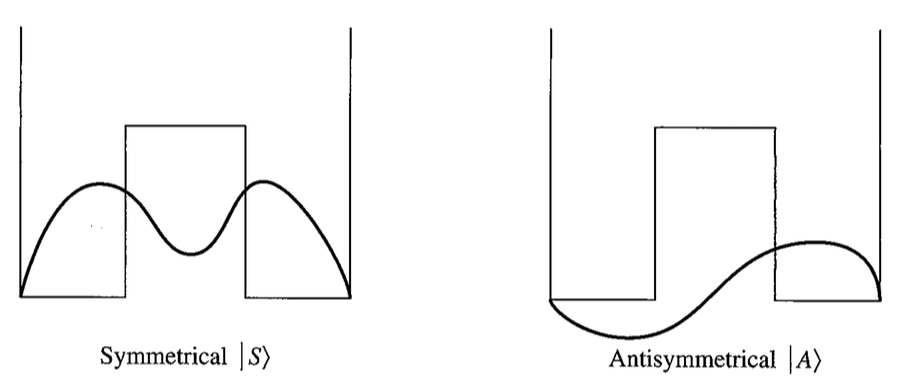
\includegraphics[width = 12.4cm]{./Sakurai/Fig_4.3.png}
\caption{对称双势阱的两个最低能量态$|S\rangle$(对称性)和$|A\rangle$(反对称性)}
\label {Fig4.3}
\end{centering}
\end{figure}

\begin{equation}
E_A>E_S
\end{equation}

\noindent 这点我们可以从图{\ref{Fig4.3}}上推断出来,因为反对称态的波函数有着更大的曲率。如果中间屏障很高的话,能量区别很小,我们后面会详细谈到相关影响。

我们可以写\footnote{译者注:这是为了凸显一些特质}

\begin{subequations}
\begin{align} \label{4.2.37a}
|R\rangle = \frac{1}{\sqrt{2}}(|S\rangle + |A\rangle)
\end{align}

\noindent 和

\begin{align} \label{4.2.37b}
|L\rangle = \frac{1}{\sqrt{2}}(|S\rangle - |A\rangle)
\end{align}
\end{subequations}

\noindent (\ref{4.2.37a})和(\ref{4.2.37b})所示的波函数,各自主要集中在右手边和左手边。它们显然不是宇称本征态,反倒是在宇称算符下互相转换。注意到它们甚至都不是能量本征态,是典型的所谓的{\textbf{非定态}}。更准确的说,假定体系在$t=0$的时候是$|R\rangle$,随时间演化后,有

\begin{equation}
\begin{split}
|R, t_0 = -;t\rangle &= \frac{1}{\sqrt{2}}\left(e^{-iE_St/\hbar}|S\rangle + e^{iE_At/\hbar}|A\rangle\right)\\
&=\frac{1}{\sqrt{2}}e^{-iE_St/\hbar}\left(|S\rangle+e^{-i(E_A-E_S)t/\hbar}|A\rangle\right)
\end{split}
\end{equation}

\noindent 在$t=T/2\equiv2\pi\hbar/2(E_A-E_S)$,系统是出于$|L\rangle$态的。在$t=T$,系统回到$|R\rangle$态,如此往复。因此,总的来说,我们可以定义系统在$|R\rangle$和$|L\rangle$之间振动,角频率为

\begin{equation}
\omega = \frac{(E_A-E_S)}{\hbar}
\end{equation}

\begin{figure}
\begin{centering}
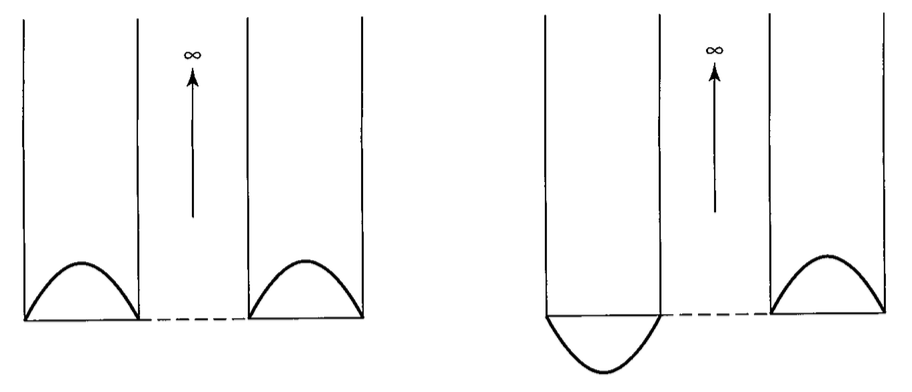
\includegraphics[width = 12.4cm]{./Sakurai/Fig_4.4.png}
\caption{对称双势阱与无穷大中间屏障}
\label {Fig4.4}
\end{centering}
\end{figure}

\noindent 这种振动行为在量子力学中也可以被视为一种“模式耦合”。一个粒子出事的时候被限制在处于右手态,它可以通过耦合穿过经典禁区进入左手态,然后再回到右手态,然后循环往复。然而,如果我们让中间的屏障无穷高,如图{\ref{Fig4.4}},这时候$|S\rangle$和$|A\rangle$这时候是简并的态,这时候(\ref{4.2.37a})和(\ref{4.2.37b})仍然是能量本征态,尽管它们并不是宇称本征态。当一个系统处于$|R\rangle$的时候,它将一直处于$|R\rangle$($|R\rangle$与$|L\rangle$之间振荡的事件变为$\infty$)。由于中间屏障无穷高,两边不能见立耦合。所以说,如果存在简并,我们物理上能理解的能量本征态不再必须是宇称本征态了。尽管有空间反演对称的哈密顿量,我们仍然可以有不对称的基态,所以在简并的情况下,能量本征态$|S\rangle$和$|A\rangle$并不必须遵守$H$的对称性。

这是一个非常简单的对称性在简并下遭到破坏的粒子。自然界中有很多这样的例子,比如铁磁体。铁原子的哈密顿量是旋转对称的,但是铁磁体却有种明确的空间指向;因此,这些基态并不是空间旋转对称的,因为自旋全都指向一些确定的(但是随意的)方向。\footnote{译者注:这是说,这个方向可以是任意方向,但一旦确定了这个方向,自旋都会大多指向这个方向。}

一个教科书级别的展示对称双势阱的粒子的重要性的例子就是氨气分子系统,如图{\ref{Fig4.5}}。我们假想三个\ce{H}原子都成一个等边三角形的三个顶点。氮原子可以在等边三角形的上边或者下边,其中上下的定义可以根据分子的转动轴来区分,如图{\ref{Fig4.5}}。氮原子的上和下态,就相当于是对称双势阱的$R$和$L$态一样。宇称本征态与能量本征态是图{\ref{Fig4.5}}中两个态如(\ref{4.2.37a})和(\ref{4.2.37b})所示的叠加态,而能量本征态的能量差造成的振动频率为$24,000MHz$——有着约$1cm$的波长,大概在微波波段。事实上,\ce{NH3}在微博散射物理中有着非常基本而重要的地位。

\begin{figure}
\begin{centering}
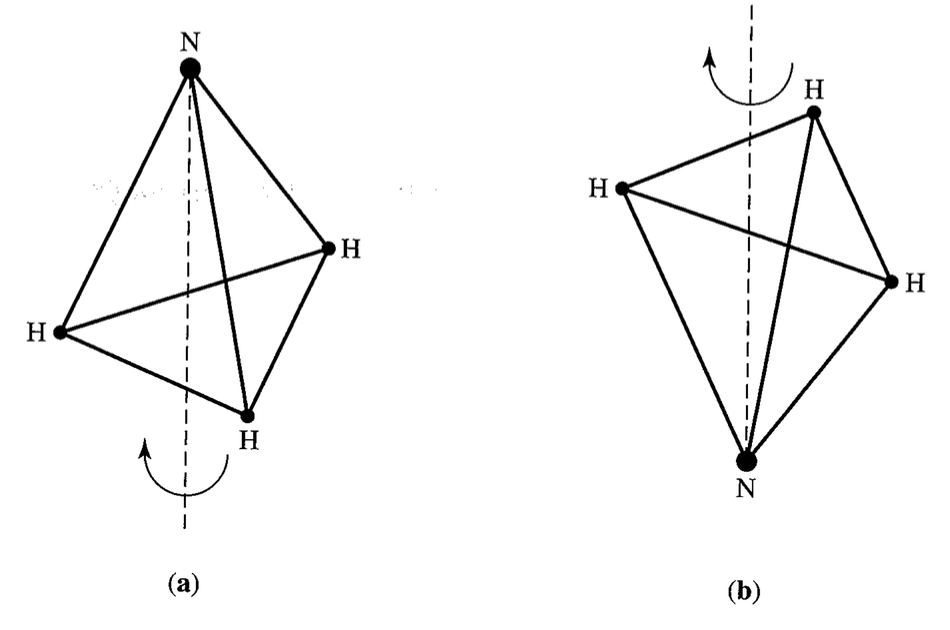
\includegraphics[width = 12.4cm]{./Sakurai/Fig_4.5.png}
\caption{一个氮气分子,\ce{NH3},其中三个\ce{H}原子处于正三角形的三个顶点上}
\label {Fig4.5}
\end{centering}
\end{figure}

自然存在的有机分子,比如氨基酸和糖,是仅仅处于$R$-型(活$L$-型)的。这种有着确定手性的分子被称为\textbf{旋光异构体}。在大多数情况下,它们的互相之间的振动周期可以认为是无穷大的——大概在$10^4$到$10^6$年的数量级。所以在任何的实际的情况中,$R-$型分子都能保持其右手性。但是令人惊奇的是,如果我们在实验室中合成这些有机分子,得到的是均等的$R$型和$L$型。为什么自然界中一种类型有着巨大的数量优势至今仍是一个谜。是因为遗传的原因,就像海螺壳一样,还是因为我们的心脏是处于左半边的呢?\footnote[1]{原注:一种想法是生命形成过程中的原子核的宇称不守恒促成了这种手性,见W. A. Booner, ``Parity Violation and the Evolution of Biomolecular Homochirality,'' \emph{Chirality}, \textbf{12} (2000) 114.}


\ \\

\noindent \textbf{宇称选择定则}

\noindent 假定$|\alpha\rangle$和$|\beta\rangle$是宇称本征态:

\begin{subequations}
\begin{align} \label{4.2.40a}
\pi|\alpha\rangle = \varepsilon_{\alpha}|\alpha\rangle
\end{align}

\noindent 和

\begin{align} \label{4.2.40b}
\pi|\beta\rangle = \varepsilon_{\beta}|\beta\rangle
\end{align}
\end{subequations}

\noindent 其中$\varepsilon_{\alpha},\, \varepsilon_{\beta}$是宇称本征值($\pm 1$)。我们有

\begin{equation}
\langle\beta|\bm{x}\alpha\rangle = 0
\end{equation}

\noindent 除非$\varepsilon_{\alpha} = -\varepsilon_{\beta}$。换句话说,奇宇称的算符$\bm{x}$连接了不同宇称的态。证明只需要利用

\begin{equation}
\langle\beta|\bm{x}|\alpha\rangle = \langle\beta|\pi^{-1}\pi\bm{x}\pi^{-1}\pi|\alpha\rangle = \varepsilon_{\alpha}\varepsilon_{\beta}(-\langle\beta|\bm{x}|\alpha\rangle)
\end{equation}

\noindent 这对于一个非零的$\langle\beta|\bm{x}|\alpha\rangle$是不可能的,除非$\varepsilon_{\alpha}$和$\varepsilon_{\beta}$拥有相反的符号。或许读者更熟悉这种形式:

\begin{equation} \label{4.2.43}
\int\psi_{\beta}^*\bm{x}\psi_{\alpha}d\tau = 0
\end{equation}

\noindent 如果$\psi_{\alpha}$和$\psi_{\beta}$有相同的宇称。这条选择定则在处理原子不同态之间的辐射跃迁的时候尤为重要,它首先由Wigner提出。辐射跃迁发生在不同宇称的态之间是多级展开的结果,我们后面会详细的讲到。这条定则可以唯相的用于分析谱线,甚至在量子力学诞生之前,那时它叫做\textbf{Laporte's rule}。Wigner表明了Laporte's rule实际上是选择定则的一个结果。

\begin{figure}[!h]
\begin{centering}
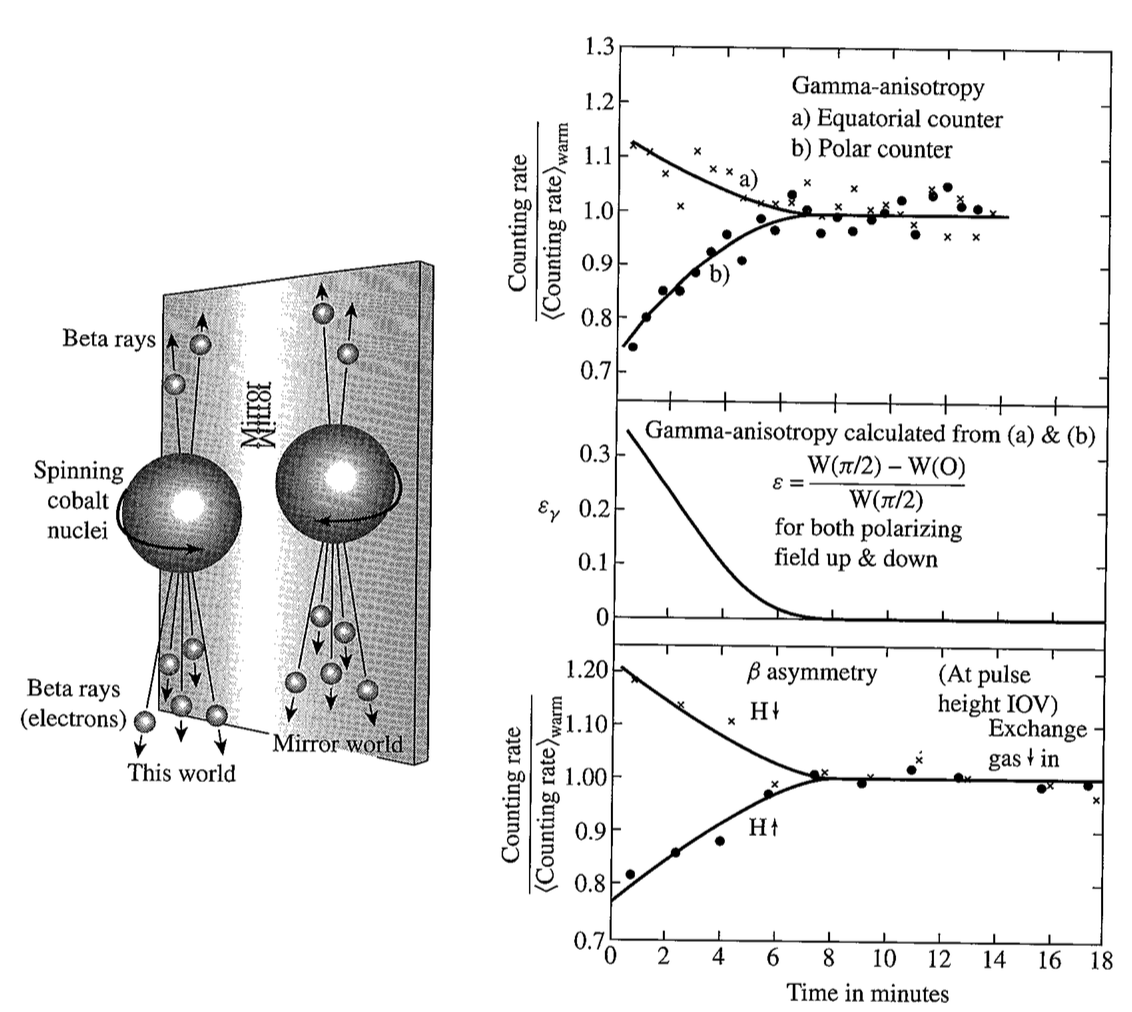
\includegraphics[width = 12.4cm]{./Sakurai/Fig_4.6.png}
\caption{实验证实的宇称不守恒。左图为最重要的观测现象——按核自旋排列的钴原子核们辐射反向电子。右方则是实验数据,表明了“向上/向下”beta衰变不对称(底部图)与核偏振程度的信号(顶部图)之间的紧密联系。随着时间演化,样品完成“锻炼”,钴原子核消偏振。(右侧数据根据Wu et al., \emph{Phys. Rev. }105 (1957) 1413 重印)}
\label {Fig4.6}
\end{centering}
\end{figure}

如果体系的哈密顿量是宇称变换下不变的,非简并能量本征态[是(\ref{4.2.43})的推论]不能有一个恒定的电偶极矩成分:

\begin{equation}
\langle n|\bm{x}|n\rangle = 0
\end{equation}

\noindent 这可以从(\ref{4.2.43}) 简单推得。基于非简并的假设,能量本征态同样也是宇称本征态[见(\ref{4.2.32})和(\ref{4.2.33})]。对于简并的态,有电偶极矩是没问题的。我们会在第{\ref{S5}}章的时候讨论线性Stark效应就是对这部分内容的应用的一个例子。

我们的这些内容可以进行推广:奇宇称的算符,就像$\bm{p}$或$\bm{S}\cdot\bm{x}$,它们的非零矩阵元只在那些有相反的宇称态的位置。相反的,偶宇称算符的非零矩阵元则在相同宇称态之间。

\ \\

\noindent \textbf{宇称不守恒}

\noindent 基本的处理称之为基本粒子之间的弱相互作用的哈密顿量则是宇称变换不守恒的。在衰变过程中,我们经常会发现体系的末态是处于不同宇称态的叠加态。诸如衰变辐射的角分布这类可观测量可以是正比于一个隗标量的,就像$\langle\bm{S}\rangle\cdot\bm{p}$。值得注意的是,知道1956年李政道和杨振宁提出宇称在弱相互作用下不守恒,并提出了重要的验证宇称守恒性的实验之前,大家都普遍认为宇称守恒是一个无暇的真理。随后的实验确实观察到了依靠隗标量(诸如$\langle \bm{S}\rangle$和$\bm{p}$之间的关联)可观测的效应。

直到今天为止,最清楚的展示宇称不守恒的实验之一仍然是最早的那个实验。实验结果,见Wu, Ambler, et al.,\emph{Phys. Rev. }\textbf{105} (1957) 1413,表明了依赖$\langle \bm{S}\rangle \cdot \bm{p}$的衰变率。在衰变过程$^{60}\ce{Co}\rightarrow\ ^{60}\ce{Ni}+e^-+\bar{\nu}_e$中,$\bm{S}$是$^{60}\ce{Co}$的核自旋,而辐射出的$e^-$的动量为$\bm{p}$。低温下制备了自旋偏振态的放射性$^{60}\ce{Co}$样品,随后在与自旋平行或者反平行的方向,观测到了辐射的$e^-$,平行还是平行取决于磁场的偏振。样品的偏振则由激发态的$^{60}\ce{Ni}$子核的$\gamma$射线的各向异性来观测(这是一个宇称守恒的效应)。实验结果如图{\ref{Fig4.6}}。经过几分钟,样品完成``预热'',观测到的$\beta$衰变的不对称性消失,走势与$\gamma$射线的各向异性的完全一致。

因为宇称在弱相互作用下并不守恒,原子核态与原子态,并不像原先想象的那样是宇称本征态,而是实际上宇称的混态。这些微妙的效应都在实验上被一一查明。

\subsection{格点平移的分立对称性}

\noindent 我们现在考虑另一种分立对称的算符,称为格点平移算符。这部分内容在固体物理里面有着十分重要的应用。

考虑一个一维周期性的势场,$V(x\pm a) = V(x)$,如图{\ref{Fig4.7}}。在现实中,我们可以考虑空间中规则分布着链状的阳离子的情况下的电子的运动。通常来讲,任意$l$的平移$\tau(l)$下哈密顿量并不一定保持不变(平移算符见节{\ref{s1.6}})。

\begin{align}
\tau^{\dagger}(l)x\tau(l) = x+l,\quad \tau(l)|x'\rangle = |x'+l\rangle
\end{align}

但当$l$恰好为周期势场的周期$a$时,我们就有

\begin{align}
\tau^{\dagger}(a)V(x)\tau(a) = V(x+a) = V(x)
\end{align}

\noindent 因为哈密顿量$H$的动能部分在任意平移下都是不变的,所以总哈密顿量满足:

\begin{align} \label{4.3.3}
\tau^{\dagger}(a)H\tau(a) = H
\end{align}

\noindent 因为$\tau(a)$是Unitary算符,从(\ref{4.3.3})中我们有

\begin{align}
\left[H,\, \tau(a)\right] = 0
\end{align}

\noindent 所以哈密顿量和$\tau(a)$可以同时对角化。尽管$\tau(a)$是Unitary的,它却不是厄米的,所以我们知道它的本征值应该是一个模长为$1$的复数。

\begin{figure}[htbp]
\begin{centering}
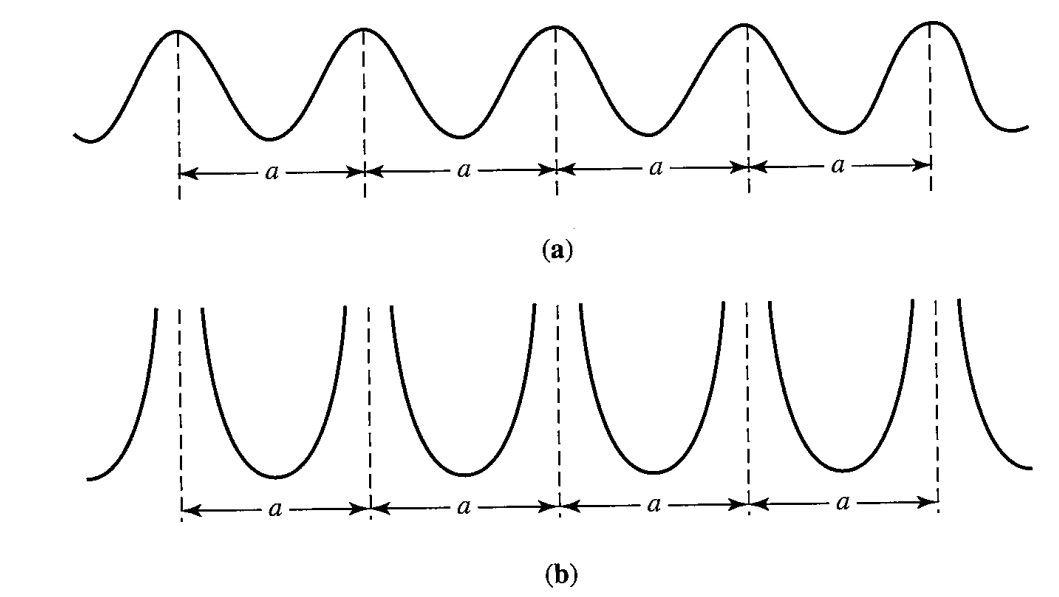
\includegraphics[width = 12.4cm]{./Sakurai/Fig_4.7.png}
\caption{(a)周期为$a$的一维周期势场图例 $(b)$一维周期势场,相邻格点间势垒无穷高的图例}
\label {Fig4.7}
\end{centering}
\end{figure}

我们希望详细计算$\tau(a)$的本征值本征态并检验其物理上的重要性,但在这之前,看一下相邻格点间势垒无穷高的周期势场的具体例子将会很有意义,如图{\ref{Fig4.7}}b。图{\ref{Fig4.7}}b的基态是怎样的呢?很明显,粒子被束缚在任意一个格点附近都是一个可能的基态。把它说的明白点,我们假定粒子被固定在第$n$个间隙,用$|n\rangle$来表示这个态。它是能量为$E_0$的能量本征态,即$H|n\rangle = E_0|n\rangle$。它的波函数$\langle x'|n\rangle$只在第$n$个间隙附近才是有限大的,其他地方都是$0$。但是,我们注意到在其它位置的态也是能量$E_0$的本征态,所以实际上有可数的无穷多个基态$n$,其中$n$从$-\infty \text{到} \infty$。

现在$|n\rangle$显然不是平移算符的本征态,因为如果我们作用一个平移算符上去,我们应该得到的是$|n+1\rangle$

\begin{align}
\tau(a)|n\rangle = |n+1\rangle 
\end{align}

\noindent 所以,尽管$\tau(a)$与$H$对易,$|n\rangle$,作为$H$的本征态,并不是$\tau(a)$的本征态。这与我们之前的那个定理一致,因为我们这里是无穷简并的。 在这种简并性之下,能量本征态就不再有体系的对称性了。随之而来的我们的任务,就是去找一个“自发” \footnote[1]{可以理解为从形式上一目了然的}的$H$和$\tau(a)$的共同本征态。

所以现在我们要回想上一节我们是如何处理类似的对称双势阱问题的。我们当时注意到了尽管$|R\rangle \& |L\rangle$都不是$\pi$的本征态,我们可以轻易的构造一个对称的和反对称的$|R\rangle \& |L\rangle$的组合形成宇称本征态。而在这里,我们的情况相当类似。我们构造一系列线性组合:

\begin{align}
|\theta\rangle \equiv \sum_{n = -\infty}^{\infty}e^{in\theta}|n\rangle
\end{align}

\noindent 其中$\theta$是一个实参数,$-\pi \le \theta \le \pi$。 可以断定$|\theta\rangle$ 自然地就是哈密顿量$H$和$\tau(a)$的本征态,$|n\rangle$有相同的能量本征值$E_0$保证了是哈密顿量的本征态。为了证明它同样也是格点平移算符的本征态,我们将$\tau(a)$作用在上面:

\begin{equation} \label{4.3.7}
\begin{split}
\tau(a)|\theta\rangle &= \sum_{n = -\infty}^{\infty} e^{in\theta}|n+1\rangle = \sum_{n = -\infty}^{\infty} e^{i(n-1)\theta}|n\rangle\\
&=e^{-i\theta}|\theta\rangle
\end{split}
\end{equation}

\noindent 注意到这一系列的本征态是由连续的参数$\theta$表示的,而且能量本征值$E_0$与$\theta$无关。

让我们回顾一下一个更看得见摸得着的情况,如图{\ref{Fig4.7}(a)},其中相邻两个格点之间的势垒不是无穷的。我们可以像之前一样构建定域的态$|n\rangle$,有$\tau(a)|n\rangle = |n+1\rangle$。但是,这次我们希望这个定域的态有可能会“漏到”相邻的格点,通过量子力学的隧穿效应。换句话说,波函数$\langle x'|n\rangle$再除了第$n$个区域附近也有一定的“余尾”。哈密顿量在这组基下对角元都相等,

\begin{align}
\langle n|H|n\rangle = E_0
\end{align}

\noindent 与$n$无关。但是,由于希望加入“泄露”,这次的哈密顿量在基$\{|n\rangle\}$下不再是对角的了。假定相邻两个位置间的壁垒很高但不是无穷高,从而我们可以让哈密顿量$H$的矩阵元中偏离对角较大的项可以忽略。因此我们认定只有两个相邻的位置有着重要的非对角项,即

\begin{align}\label{4.3.9}
\langle n'|H|n\rangle \neq 0 \quad \text{除非} \quad n' = n \quad \text{或} \quad n' = n\pm1
\end{align}

\noindent 在固体物理学里面,这种假定被称为紧束缚近似\footnote{\textbf{tight-binding approximation}}。我们定义

\begin{align}
\langle n\pm 1|H|n\rangle = -\Delta
\end{align}

\noindent 显然,由于哈密顿量的平移对称性,$\Delta$ 仍然与$n$无关。考虑到在$n\neq n'$的时候他们是彼此正交的,我们有

\begin{align}
H|n\rangle = E_0|n\rangle - \Delta|n+1\rangle - \Delta |n-1\rangle
\end{align}

\noindent 注意,这时候$|n\rangle$ 不再是能量本征态。

就像我们处理图{\ref{Fig4.7}b}那样,我们构造一组线性组合

\begin{align}\label{4.3.12}
|\theta\rangle = \sum_{-\infty}^{\infty}e^{in\theta}|\theta\rangle
\end{align}

\noindent 显然,$|\theta\rangle$是平移算符的本征态因为我们仍可以沿用(\ref{4.3.7})的推导。很自然的,我们会问一个问题,$|\theta\rangle$是不是能量本征态呢?为了回答这个问题,我们用$H$作用在上面:

\begin{equation}\label{4.3.13}
\begin{split}
H\sum e^{in\theta}|n\rangle &= E_0 \sum e^{in\theta}|n\rangle - \Delta \sum e^{in\theta}|n+1\rangle - \Delta\sum e^{in\theta}|n-1\rangle\\
&=E_0\sum e^{in\theta}|n\rangle - \Delta\sum(e^{in\theta - i\theta} + e^{in\theta + i\theta})|n\rangle\\
&= (E_0 - 2\Delta\cos\theta)\sum e^{in\theta}|n\rangle
\end{split}
\end{equation}

\noindent 与之前最大的不同的是,这回的能量本征值依赖于一个连续的参数$\theta$。 随着$\Delta$变大,简并被逐渐拉开,我们有了一个能级从$E_0-2\Delta$到$E_0+2\Delta$的连续分布。图{\ref{Fig4.8}}我们示意了随着$\Delta$从$0$开始变大,能级如何变成一个连续的能带的。

为了了解参数$\theta$的物理意义,我们来研究一下波函数$\langle x'|\theta\rangle$。平移运算下的波函数是$\tau(a)|\theta\rangle$,我们有

\begin{align}
\langle x'|\tau(a)|\theta\rangle = \langle x'-a|\theta\rangle
\end{align}

\noindent 通过让$\tau(a)$作用在$\langle x'|$上。但是同样的,我们也可以让平移算符$\tau(a)$作用在$|\theta\rangle$上,就像(\ref{4.3.7})那样。因此

\begin{align}
\langle x'|\tau(a)|\theta\rangle = e^{-i\theta}\langle x'|\theta\rangle
\end{align}

\noindent 因此

\begin{align}
\langle x'-a|\theta\rangle = \langle x'|\theta\rangle e^{-i\theta}
\end{align}

\noindent 通过下列变换我们来解这个方程:

\begin{align}\label{4.3.17}
\langle x'|\theta\rangle = e^{ikx'}u_k(x')
\end{align}

其中$\theta = ka$,$u)k(x’)$ 是一个周期性函数,周期为$a$,我们可以简单地通过代入法进行验证

\begin{align}\label{4.3.18}
e^{ik(x’-a)}u_k(x’-a) = e^{ikx’}u_k(x’)e^{-ika}
\end{align}

\begin{figure}[htbp]
\begin{centering}
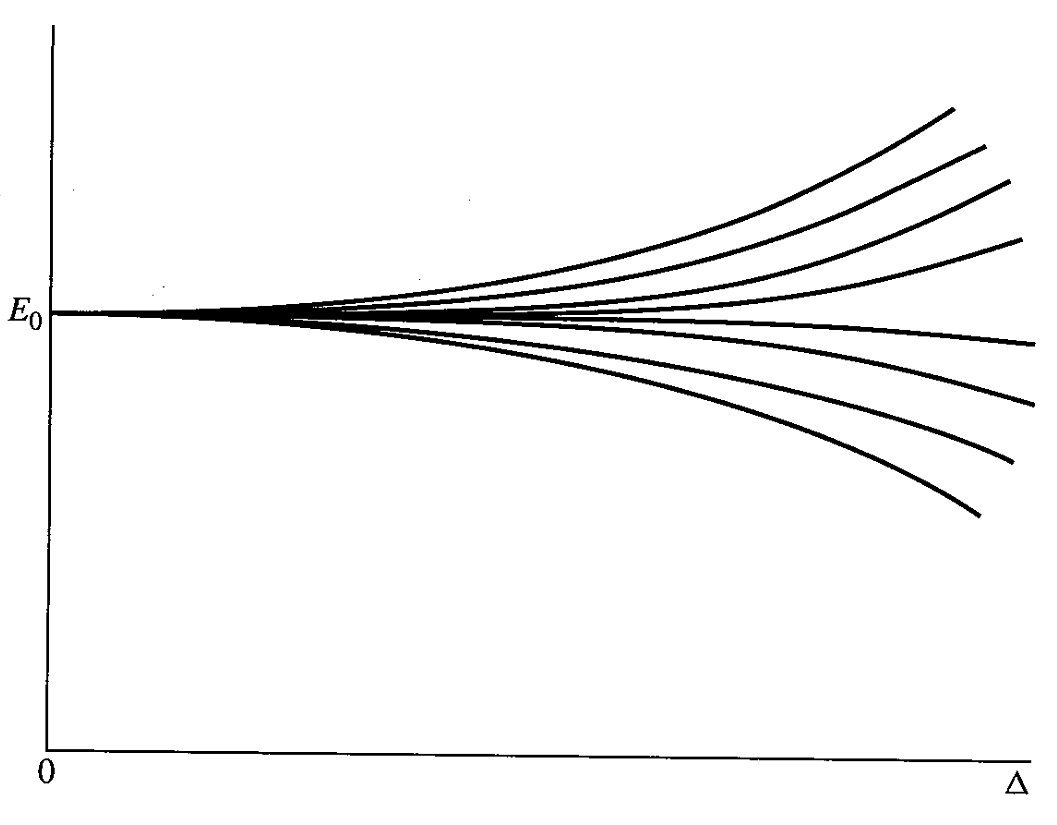
\includegraphics[width = 12.4cm]{./Sakurai/Fig_4.8.png}
\caption{随着$\Delta$的增加,能级组成了一条连续的能带}
\label {Fig4.8}
\end{centering}
\end{figure}

至此,我们得到了重要的\bf{Bloch定理}:平移算符$\tau(a)$的本征态,波函数$|\theta\rangle$可以通过平面波#e^{ikx’}$乘上一个周期函数展开。注意到我们在这个过程中只用到了#|\theta\rangle$是平移算符#\tau(a)$本征值为$e^{-i\theta}$的本征态[见\eqref{4.3.7}]。更近一步的说,这条定理在集市紧束缚近似\eqref{4.3.9}不再成立的时候也还是正确的。

我们现在要去解释我们先前的由\eqref{4.3.13}得到的关于\eqref{4.3.12}$|\theta\rangle$的结果。我们知道波函数可以用波矢为$k$的空间中传播的平面波通过周期函数$u_k(x’)$调制得到[见\eqref{4.3.17}]。在$\theta$从$-\pi$到$\pi$变化的时候,波矢从$-\pi/1$变化到$\pi/a$。能量本征值$E$就有关于$k$的如下关系

\begin{align}\label{4.3.19}
E(k) = E_0-2\Delta\cos ka
\end{align}

需要注意能量本政治方程只要紧束缚条件成立就与势能的具体形式没有关系。同时也需要注意在$|k|=\pi/a$的地方,Bloch波函数\eqref{4.3.17}有一个截断。方程\eqref{4.3.19}定义了色散曲线,如图\ref{Fig4.9}。由于隧穿,不可数无穷多的简并被彻底地消除了,而得到了一个连续的能带,从$E_0-2\Delta$到$E_0+2\Delta$,被称为\bf{Brillouin区}。

现在为止我们只考虑了单粒子在周期势中运动的结果。在更贴近现实的情况中,我们必须要考虑非常多的电子在这个势众运动的行为。事实上,电子需要满足Pauli不相容原理(我们将在第\ref{Chap7}章中详细说明),所以将会填充能带。在这样的分析下,金属、半导体等物质的主要定性结论可以通过评议不变性以及不相容原理来进行理解。

读者或许注意到了节\ref{Sec4.2}中对称双势井问题和本节中周期势问题的相似性。对比图\ref{Fig4.3}和图\ref{$.3},我们注意到它们可以视为势能包含有限个谷的两个不同的极端情况(2 vs 无穷)。

\begin{figure}[htbp]
\begin{centering}
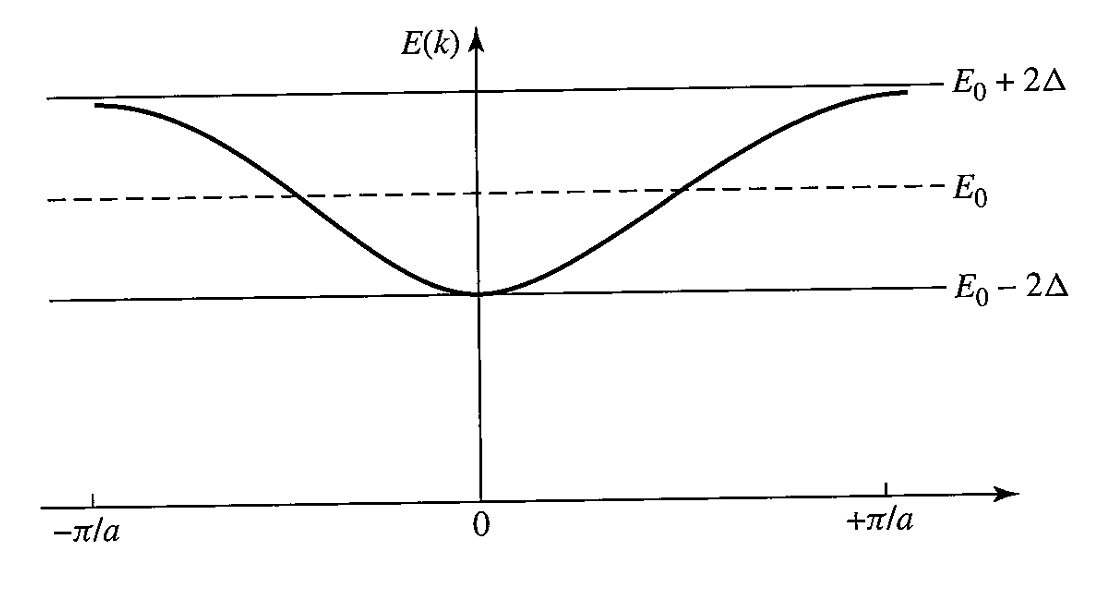
\includegraphics[width = 12.4cm]{./Sakurai/Fig_4.9.png}
\caption{在Brillouin区$|k|\le\pi/a$中,$E(k) \text{vs.} k$的色散关系。}
\label {Fig4.9}
\end{centering}
\end{figure}



\subsection{时间反演的分立对称性}

这一节我们研究另一种分立对称性——时间反演对称性。这是一个很新的并且难于讲述的话题,有一定程度上要怪这个名字(时间反演)的问题,它让我们想起科幻小说。我们这一节干的事情或许可以用“运动的反演”\footnote{reversal of motion}来更好的描述。事实上,这才是时间反演方面的开山祖师E. Winger在1932年完成那篇奠基性的论文的时候所使用的词。

\begin{figure}[htbp]
\begin{centering}
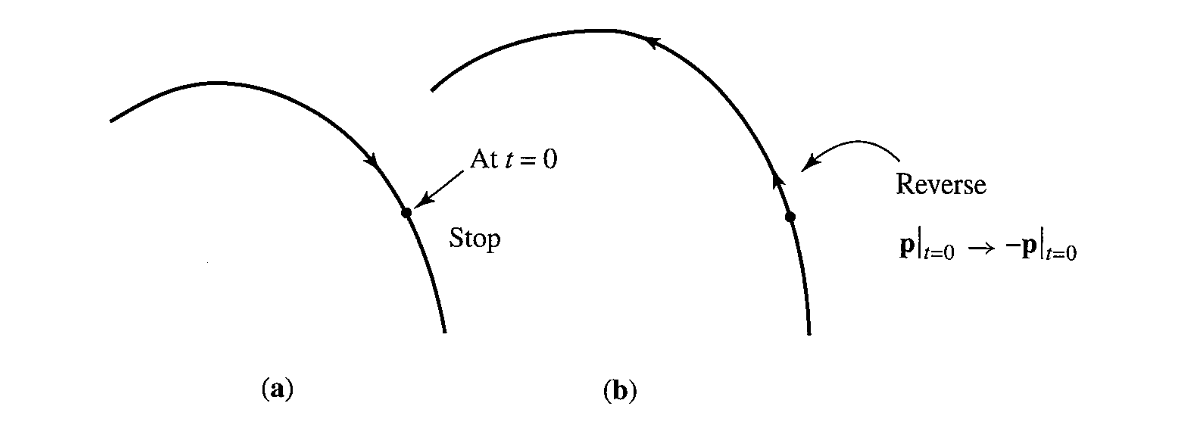
\includegraphics[width = 12.4cm]{./Sakurai/Fig_4.10.png}
\caption{(a) 在$t=0$停止的经典轨迹 (b) 它在进行$\bm p|_{t=0}\rightarrow-\bm p|_{t=0}$之后的运动}
\label {Fig4.10}
\end{centering}
\end{figure}

\end{document}
